\chapter{Diskussion der Umsetzung}
\label{chap:five}
Im folgendem Kapitel wird das Design des Prototypen besprochen und die Teilsysteme vorgestellt und skizziert wie die Teilsysteme
funktionieren. Dabei wird exemplarisch anhand von einzelnen Methoden der Klassen oder Funktionen beschrieben wie das funktioniert
Im Quellcode selber wird ausführlich jede Methode beschrieben.
\section{Implementierung}
    \subsection{Technische Details der Implementierung}
    Das Proof-of-Concepts wurde mittels der Programmiersprache Python umgesetzt.
    Python ist eine höhere Programmiersprache. Sie ist weitverbreitet \cite[vgl.][]{loukides_where_2021} und besitzt
    eine einfache Syntax. Besonderheiten von Python sind der Verzicht auf geschweifte Klammern und Interpunktionen nach Anweisungen.
    Die Anweisungen sind dagegen durch Einrückungen strukturiert und nicht durch öffnende und schließende Klammern
    getrennt. Des Weiteren zeichnet sich Python durch eine dynamische Typisierung aus und ist dadurch für Skripte als auch 
    für die schnelle Entwicklung von Anwendungen geeignet. Python erlaubt die Aufteilung von Programmen in Modulen, die in anderen Python-Programmen wiederverwendet werden können
    \cite[vgl.][]{python_6_2021}.
    Sie ist für alle wichtigen Plattformen frei verfügbar und besitzt eine große Dokumentation \cite[vgl.][]{python_welcome_2021}.
    Wie andere Programmiersprachen besitz Python eine umfangreiche Standardbibliothek. 
    Dazu gibt es noch eine Vielzahl von Modulen, Programmen und Werkzeugen von Drittanbietern \cite[vgl.][]{python_pypi_2021}.
    
    
    Genutzt wurde für das Projekt insbesondere die Python-Bibliothek pandas, die eine Open-Source-Bibliothek für Datenanalyse und 
    Datenmanipulation darstellt \cite[vgl.][]{pandas_pandas_2021}. 
    Wichtige Konzepte dieser Bibliothek sind der pandas Dataframes und die pandas Series, die pandas Objekte sind. Der pandas Dataframe ist eine zweidimensionale 
    tabellarische Datenstruktur mit beschrifteten Achsen (Spalten und Reihen). In ihn
    werden die Daten unter anderem aus csv- oder xlsx-Dateien über pandas Funktionen geladen.
    Eine pandas Series kann Bestandteil eines Dataframes sein. Der Datentyp entspricht eines eindimensionales Arrays. \autoref{fig:pandas Dataframe und pandas Series} zeigt anhand der Umsatzdaten die ersten fünf Reihen
    eines pandas Dataframe und einer pandas Series desselben Dataframes. Zugriff auf die Series erfolgt über
    den Spaltenkopf 'Lieferant Abk.' der als ein Schlüssel zur Series dient. Sowohl der Dataframe als auch die Series haben einen Index, 
    über den auf die einzelnen Werte zugegriffen werden kann. 
    
    
    \begin{figure}[h]
        \centering
            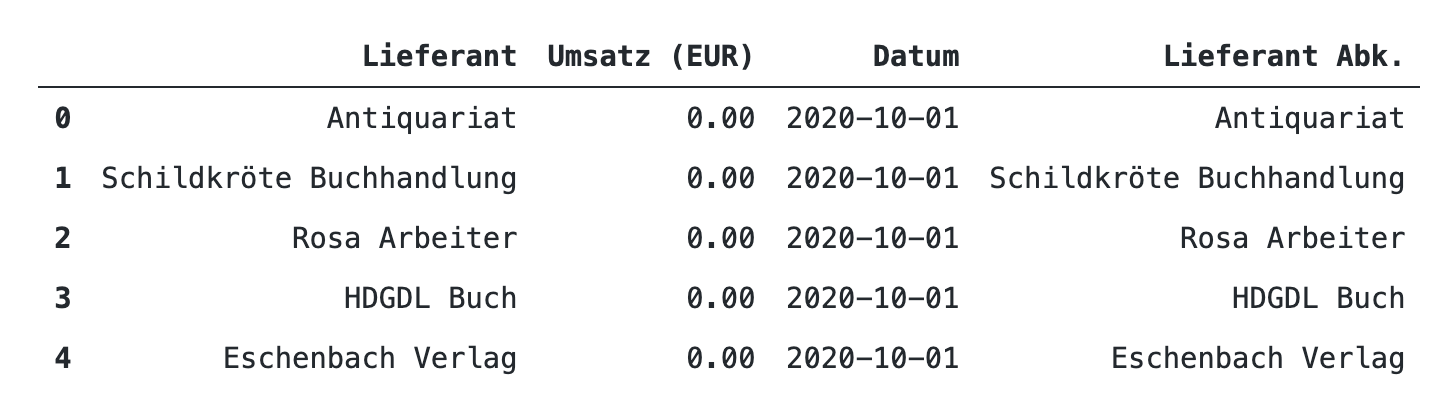
\includegraphics[width=7.5cm, height=3.0cm]{dataframe_example}
            \hspace{1cm}
            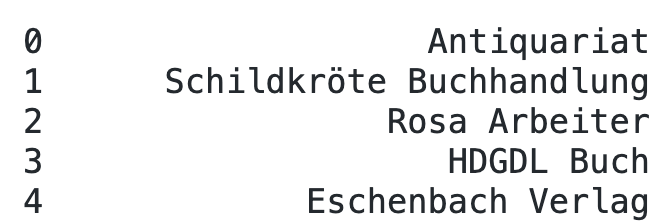
\includegraphics[width=5.0cm, height=3.0cm]{series_example}
            \caption{pandas Dataframe und pandas Series}
            \label{fig:pandas Dataframe und pandas Series}
    \end{figure}
    
    Auf dem Dataframe, der als sogenannter Container für die Series dient, können verschiedene Operationen der Datenanalyse und 
    -manipulation erfolgen. Ähnlich wie bei Abfragen einer Datenbank lassen sich verschiedene Funktionen wie \texttt{sort()}- oder \texttt{groupby()}-Funktionen in Zusammenhang
    mit Aggregatfunktionen wie \texttt{mean()}, \texttt{median()} oder \texttt{sum()} auf den Series durchführen.
    Auch gibt es eine Vielzahl von Funktionen, um die Daten rasch zu explorieren. Die Werte der Zellen können verschiedene Datentypen
    annehmen. Zum Beispiel können die Datumswerte der Spalte 'Datum' in \texttt{datetimeformat-Objekte} umgewandelt werden.

    In Verbindung mit pandas ist Python neben \textsf{R} und Matlab im wissenschaftlichen Kontext für Data-Science-Projekte sehr beliebt.
    
    Es gibt eine Vielzahl an Bibliotheken für Python, die für die Entwicklung von interaktiven Datenvisualisierungen verfügbar sind. Zu
    nennen wären Bokeh \cite[vgl.][]{van_de_ven_bokeh_2021}, Altair \cite[vgl.][]{altair_altair_2021} und die 
    Graphic Libraries von Plotly \cite[vgl.][]{plotly_plotly_2021}. Für das Projekt wurde sich für Plotly Express entschieden 
    und dieses hauptsächlich genutzt. 
    Plotly Express ist eine Graphische Bibliothek für Python, \textsf{R} und Javascript. Es ist eine Weiterentwicklung der Bibliothek Plotly Graphic Objects. 
    Plotly Express besitzt eine einfachere Syntax bei fast annäherender Feature-Gleichheit mit Plotly Graphic Objects. So können mit wenigen Zeilen Python-Code interaktive Grafiken erzeugt werden. 
    An interaktiven Basisfunktionalitäten bietet Plotly Express zum Beispiel Hover-Informationen der Datenpunkte, Zoom-In und Zoom-Out-Möglichkeiten,
    das Aus- und Abwählen von Balken oder Linien in den entsprechenden Diagrammen. Plotly Express kann pandas Dataframes 
    oder pandas Series als Datenobjekte erwarten und verarbeiten. Dabei können die Spaltenköpfe die Achsen darstellen 
    und die einzelnen Werte der Spalten die Datenpunkte bilden.Die Rendering-Engine für die Diagramme beruht auf dem JavaScript Framework D3.js. 
    Plotly Express ist frei verfügbar. In Kombination mit der Bibliothek Dash für die Entwicklung von interaktiven Dashboards lässt sich Plotly Express gut anwenden, 
    da beide von der selben Firma entwickelt werden. Mit der Bibliothek Dash wurde das Dashboard realisiert.
    
    Dash baut auf den Technologien Flask, Plotly.js und React.js auf. Das Framework ermöglicht die Erstellung interaktiver Webapplikationen 
    oder 'Analytical Applications' in Python ohne Javascript programmieren zu müssen \cite[vgl.][]{plotly_dash_2021}.
    Es gibt verschiedene Dash-Komponenten, die unterschiedliche Funktionen erfüllen. \texttt{Dash\_html\_components} stellen Klassen für alle HTML-Tags bereit.
    Die Schlüsselwortargumente dieser Komponente beschreiben HTML-Attribute wie style, className und id \cite[vgl.][]{plotly_dash_2021-2}. 
    Andere Komponenten sind \texttt{dash\_core\_components} oder \texttt{dash\_dependencies} \cite[vgl.][]{plotly_dash_2021-1}. Während die \texttt{dash\_core\_components}
    Steuerelemente und Graphen erzeugen, regeln die \texttt{dash\_dependencies} über Callback-Decorator-Funktionen die Interaktion zwischen den einzelnen Komponenten.
    So kann zum Beispiel in der Dash-WebApplikation das Verhalten eines Diagramms von den Werten eines Dropdown-Menu gesteuert werden. 
    Die zugehörige Callback-Decorator-Funktion wird in diesem Falle automatisch von Dash aufgerufen, sobald sich der Wert des Dropdown-Menüs ändert. 
    Dabei bewältigt Dash alle Javascript-Anforderungen im Front- und im Backend \cite[vgl.][]{plotly_dash_2021-3}.
    \texttt{Dash\_bootstrap\_components} ist eine weitere Bibliothek, die zum Einsatz in diesem Projekt kommt. Sie unterstützt die grafische Umsetzung
    des Dashboardes \cite[vgl.][]{faculty_dash_2021}.

    \autoref{tab:Software-Requirements} zeigt nochmals einen 
    kurzen Überblick über die Versionsnummern der genutzten Programmiersprache und der hauptsächlich genutzten Bibliotheken sowie deren Open-Source
    Lizenzen.
    
    \begingroup
        \setlength{\tabcolsep}{4pt} % Default value: 6pt
        \renewcommand{\arraystretch}{1.5}
        %\resizebox{\textwidth}{!}{
        \begin{table}[h]
            \centering
            \begin{adjustbox}{max width=\textwidth}
            \Huge
            \begin{tabular}{lccl}
              %\begin{tabular}{p{3cm}p{5cm}p{1cm}p{1.5cm}p{2cm}p{4cm}}
               \toprule
               \textbf{Name}             &{Version}    &\textbf{Lizenz}                        & \textbf{Webseite}\\
               \midrule     
                    Python               &3.7.9         &Open Source (PSF)                     & \url{https://docs.python.org/3.7/}\\
                    pandas               &1.1.5         &3-Clause-BSD-License                  & \url{https://pandas.pydata.org/pandas-docs/version/1.1.5/}\\
                    Plotly               &4.14.14       &MIT-License                           & \url{https://plotly.com/python/}\\
                    Dash                 &1.18.1        &MIT-License                           & \url{https://dash.plotly.com/}\\


                \bottomrule
            \end{tabular}
            \end{adjustbox}
            \caption
            \label{tab:Software-Requirements}
            }
             \end{table}
        \endgroup
    
     
    \subsection{Systemarchitektur}
    
    Das System teilt sich in drei Teilsysteme auf, die im \autoref{chap:five_one_three} näher beschrieben werden. 
    \autoref{tab:Teilsysteme} zeigt die drei Teilsysteme mit einer Kurzbeschreibung der Hauptaufgabe.
    Teilsystem 1 ist für die erste Bereinigung der Daten und den Import der Daten in ein einheitliches Datenformat verantwortlich. 
    Teilsystem 2 greift auf den Speicherort der importierten Dateien zu und bereitet die Daten für die Anzeige im Dashboard vor, 
    indem es mit pandas Daten vorfiltert, gruppiert und Berechnungen auf den Daten ausführt. Teilsystem 3 ist für das Layout des Dashboards, 
    die Erstellung der Diagramme, die Anordnung der Diagramme, die Bereitstellung von Interaktionen mit dem Dashboard im Frontend
    verantwortlich. Teilsystem 1 und Teilsystem 2 wurden versucht objektorientiert zu programmieren, da hier der Anspruch bestand, den Programmcode
    für verschiedene Daten wiederzuverwenden. Teilsystem 3 besteht vorerst nur aus Funktionen, die die Anzeige im Frontend ermöglichen.
    %Teilsystem 4 besteht dahingegen wieder aus objekt-orientierter Programmierung. Genutzt wird hier eine Library, die OOP vorgibt. 

       \begingroup
            \setlength{\tabcolsep}{4pt} % Default value: 6pt
            \renewcommand{\arraystretch}{1.5}
            %\resizebox{\textwidth}{!}{
            \begin{table}[h]
                \centering
                \begin{adjustbox}{max width=\textwidth}
                \Huge
                \begin{tabular}{cll}
                  %\begin{tabular}{p{3cm}p{5cm}p{1cm}p{1.5cm}p{2cm}p{4cm}}
                   \toprule
                   \textbf{Teilsystem}             & Name   &{Hauptaufgabe} \\
                   \midrule     
                            1                      &Import  &Import und erste Bereinigung der Daten aus heterogenen Datenquellen.\\
                            2                      &Datenbearbeitung     &Aufbereitung der Daten für die graphische Darstellung im Dashboard.\\
                            3                      &Darstellung          &Umwandlung der Daten in Datenvisualisierungen, etc. und Anzeige im Dashboard.\\
                        %   4                      &Standardbericht      &Export ausgewählter Datenvisualisierungen und Darstellung in Berichtsform.\\

                    \bottomrule
                \end{tabular}
                \end{adjustbox}
                \caption
                \label{tab:Teilsysteme}
                }
                 \end{table}
            \endgroup
    

    \subsection{Teilsysteme}
    \label{chap:five_one_three}
    \textit{Teilsystem 1 Import}\\
    Das Teilsystem Import ist verantwortlich für den Import der Daten im Rohformat aus vordefinierten Importverzeichnissen 
    in vordefinierte Zielverzeichnisse. Das Ziel ist einerseits die Daten automatisch ohne Informationsverlust zu importieren 
    und andererseits diese mit notwendigen Daten für die weitere Analyse anzureichern und erste Bereinigungen der Daten durchzuführen. Die Daten werden zum Abschluss in 
    csv-Format abgespeichert. Mit dem Teilsystem soll eine einheitliche Datengrundlage für die spätere Bearbeitung
    und Darstellung garantiert werden.
    Für das csv-Format wurde sich aufgrund seiner flachen und einfachen Struktur, der guten Lesbarkeit
    und seiner weiten Verbreitung entschieden.
    % Die Daten werden jeweils in ein pandas Dataframe geladen. Das Dataframe wird dann verschiedentlich bearbeitet, bevor es zum Schluss als csv-Datei in dem jeweiligen
    % Zielverzeichnis abgespeichert wird.
    Das Teilsystem Import besteht aus vier Klassen. Die \autoref{fig:classes import} zeigt die einzelnen Klassen mit ihren Methoden.
    Die Klassen im Teilsystem Import sind auf die Daten aus fremden Quellen zugeschnitten
    (Budget Umsatz, Neuerwerbungslisten, Ausleihe (Anwendungsfall 2, 4-6)). Dennoch können mit mit ihnen auch die bibliotheksinternen Daten
    wie Lesesaalnutzung (Anwendungsfall 3) bearbeitet werden. 
    \begin{figure}[H]
        \centering
            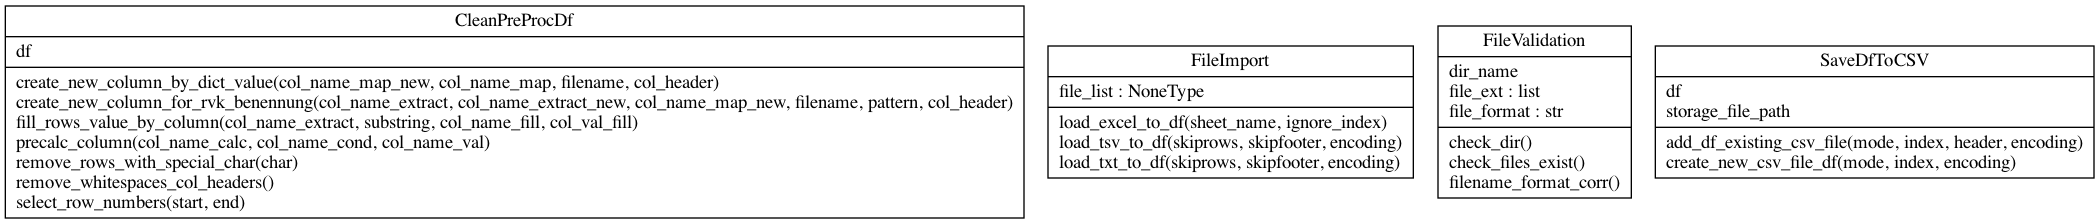
\includegraphics[width=14cm, height=2.5cm]{classes_imp}
            \caption{Klassendiagramm - Teilsystem Import}
            \label{fig:classes import}
    \end{figure}

    Instantiiert werden die einzelnen Klassen für die jeweiligen konkreten bibliothekarischen Daten in eigenen Skripten. 
    So gibt es Skripte für Budget, Umsatz, Ausleihe und Bestand/Neuerwerbungen. Diese verwenden für die Daten passende Methoden.
        
    Den Ablauf des Teilsystems zeigt schematisch die \autoref{fig:flow import}.

    \begin{figure}[H]
        \centering
            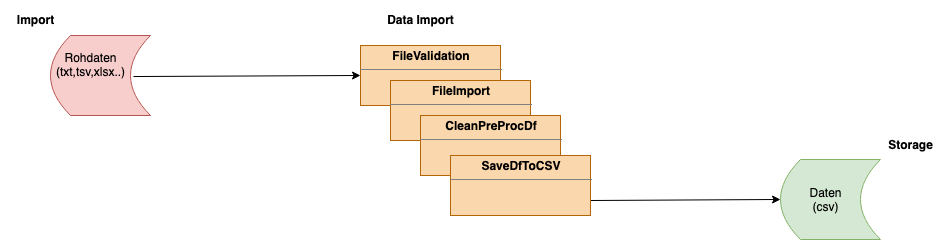
\includegraphics[width=12cm, height=2.5cm]{flow_imp}
            \caption{Datenfluss - Teilsystem Import}
            \label{fig:flow import}
    \end{figure}

    
    (1) Für den ersten Schritt sind die Klassen \texttt{FileValidation} und \texttt{FileImport} verantwortlich.
    Die Dateien werden aus einem vorher definierten lokalen Verzeichnis in ein pandas Dataframe geladen. 
    Dabei wird mit Methoden der Klasse \texttt{FileValidation} sichergestellt, dass sowohl das Verzeichnis als auch die Dateien existieren. 
    Des Weiteren wird sichergestellt, dass die Dateinamen einem definierten semantischen Format wie dem Datuumsformat YYYY\_MM\_DD und 
    einem Dateiformat wie txt, xlsx oder tsv entsprechen. Wenn die Daten nicht diesen Vorgaben entsprechen, werden sie nicht
    importiert. Da die Daten unterschiedlich aufgebaut und in unterschiedlichen Dateiformaten vorliegen 
    werden beim Import in den pandas Dataframe jeweils verschiedene Methoden angewandt.
    
    Beim Ladeprozess der Dateien in den pandas Dataframe wird mit den Methoden \texttt{load\_txt\_to\_df} oder \texttt{load\_tsv\_to\_df} der Klasse \texttt{FileImport} 
    der Dateiname von der Datei extrahiert und in einer neu geschaffenen Spalte des Dataframes im Datumsformat YYYY-MM-DD gespeichert.
    Anhand den Werten dieser Spalte werden später verschiedene Datenanalysen und Datenvisualisierungen vollzogen. \footnote{Dieses Verfahren wird bei den Daten ausgeführt, die einer zusätzlichen Datumsspalte bedürfen.} 
    Verantwortlich für die Extrahierung des Dateinamens ist die in \texttt{utils.py} ausgelagerte Funktion \texttt{date\_from\_filename},
    die den Dateinamen als Argument entgegennimmt.
    \footnote{In der Datei \texttt{utils.py} sind noch andere Funktionen als stand-alone-functions für den Datenimport und Datenbearbeitung gruppiert,
    da diese das Objekt \texttt{self} nicht verändern.} 
    
    (2) Das geladene pandas Dataframe wird im zweiten Schritt durch die Klasse \texttt{CleanPreProcDf} aufgenommen und durch verschiedene Methoden dieser Klasse
    manipuliert. Beispielhaft ist hier die Methode \texttt{create\_new\_column\_for\_rvk\_benennung} zu nennen, die aus der Spalte der Signatur 
    der Neuerwerbungen die Hauptklassen der \textit{\acrlong{RVK}} extrahiert und in einer neuen Spalte speichert. Dieser Methode liegt eine csv-Datei
    der \textit{\acrshort{RVK}} zu Grunde, die mit einem Skript aus der \textit{\acrshort{RVK}}-XML-Datei entstanden ist. Manuell ergänzt wurde diese 
    noch um selbstgeschaffene Hauptklassen der Institutsbibliothek. Die Methode wird sowohl bei den Neuerwerbungs- und Ausleihdaten angewendet.
    Ebenso entstehen neue Spalten bei Umsatz- und Budgetdaten. In Bezug auf die Darstellung der Daten im Dashboard werden
    hier die Namen der Lieferanten und Kostenstellen in lesbarer Form in einer neuen Spalte gespeichert. 
    Des Weiteren gibt es in der Klasse Methoden, die für die Entfernung von Reihen mit bestimmten syntaktischen Zeichen wie Bindestrichen verantwortlich sind oder 
    die unnötige Leerzeichen in Spaltenköpfen löschen und mit einem Leerzeichen ersetzen.
    Ferner werden erste Berechnungen auf den Daten ausgeführt, um valide Daten für die Auswertung zu haben. Dies betrifft die Ausleihdaten und wird durch die
    Methode \texttt{precalc\_column} realisiert.
    \footnote{Im Arbeitsprozess der Medienerschließung validiert die Bibliothek die RFID-Etiketten der Medien durch einmalige Ausleihe der Medien am Selbstverbucher.
    Deswegen wird die Anzahl der Ausleihe pro Medium um eins reduziert.}
     
    (3) Nachdem Transformationsprozess wird das veränderte pandas Dataframe als csv-Datei in einem vorher definierten Zielordner gespeichert. 
    Verantwortlich ist dabei die Klasse \texttt{SaveDFToCSV} mit den zwei Methoden \texttt{add\_df\_existing\_csv\_file create\_new\_csv\_file\_df}. 
    Die je nach dem mit dem Dataframe eine neue csv-Datei erstellen oder an eine bereits vorhandene csv-Datei den Dataframe anhängen.
    \autoref{fig:umsatzuebersicht_csv} zeigt anhand einer Umsatz-Datei, die im txt-Format gespeichert ist, die Transformation von diesem Format 
    in ein csv-Format. Für die lesbare Darstellung wird die csv-Datei in einem Tabellenformat angezeigt.

    \begin{figure}[h]
        \centering
            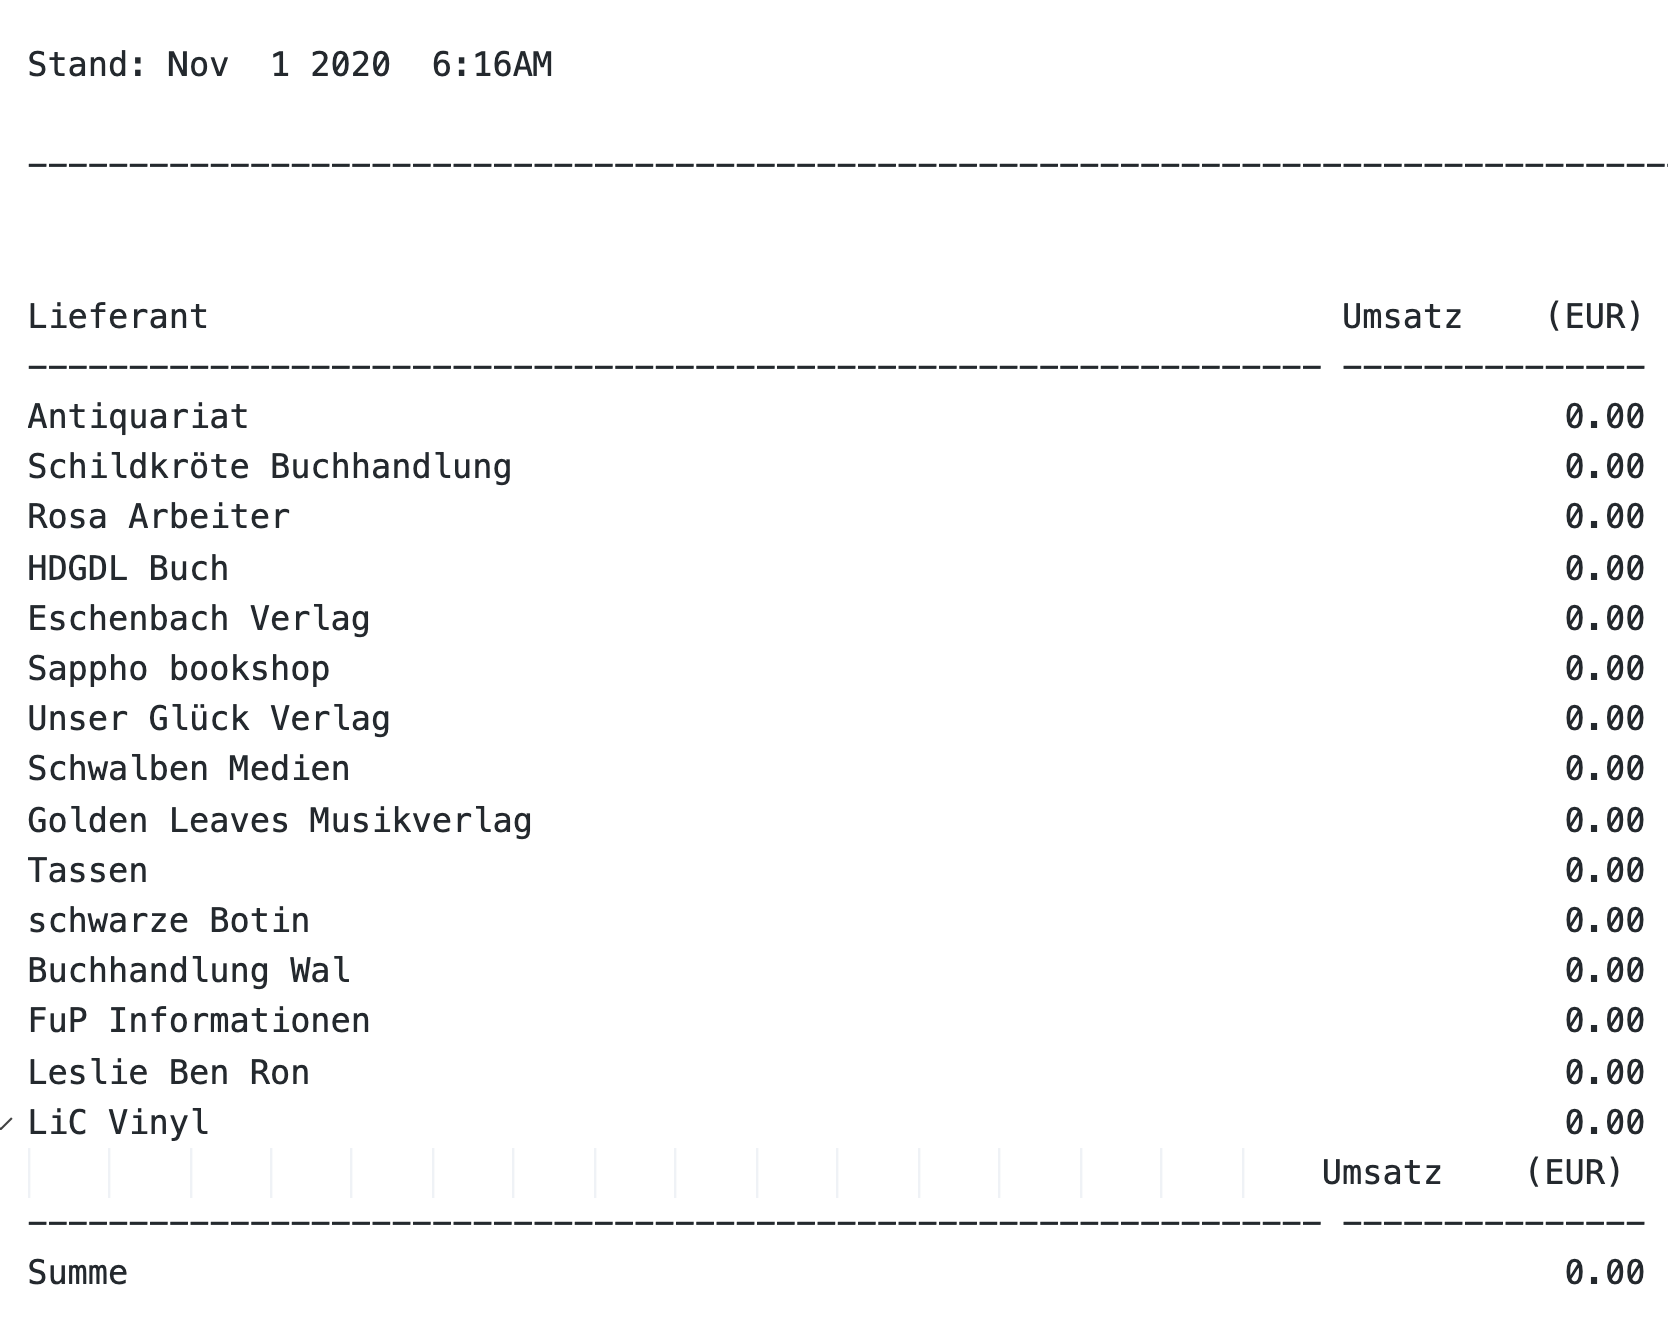
\includegraphics[width=6.5cm, height=7.0cm]{umsatzuebersicht_mtl}
            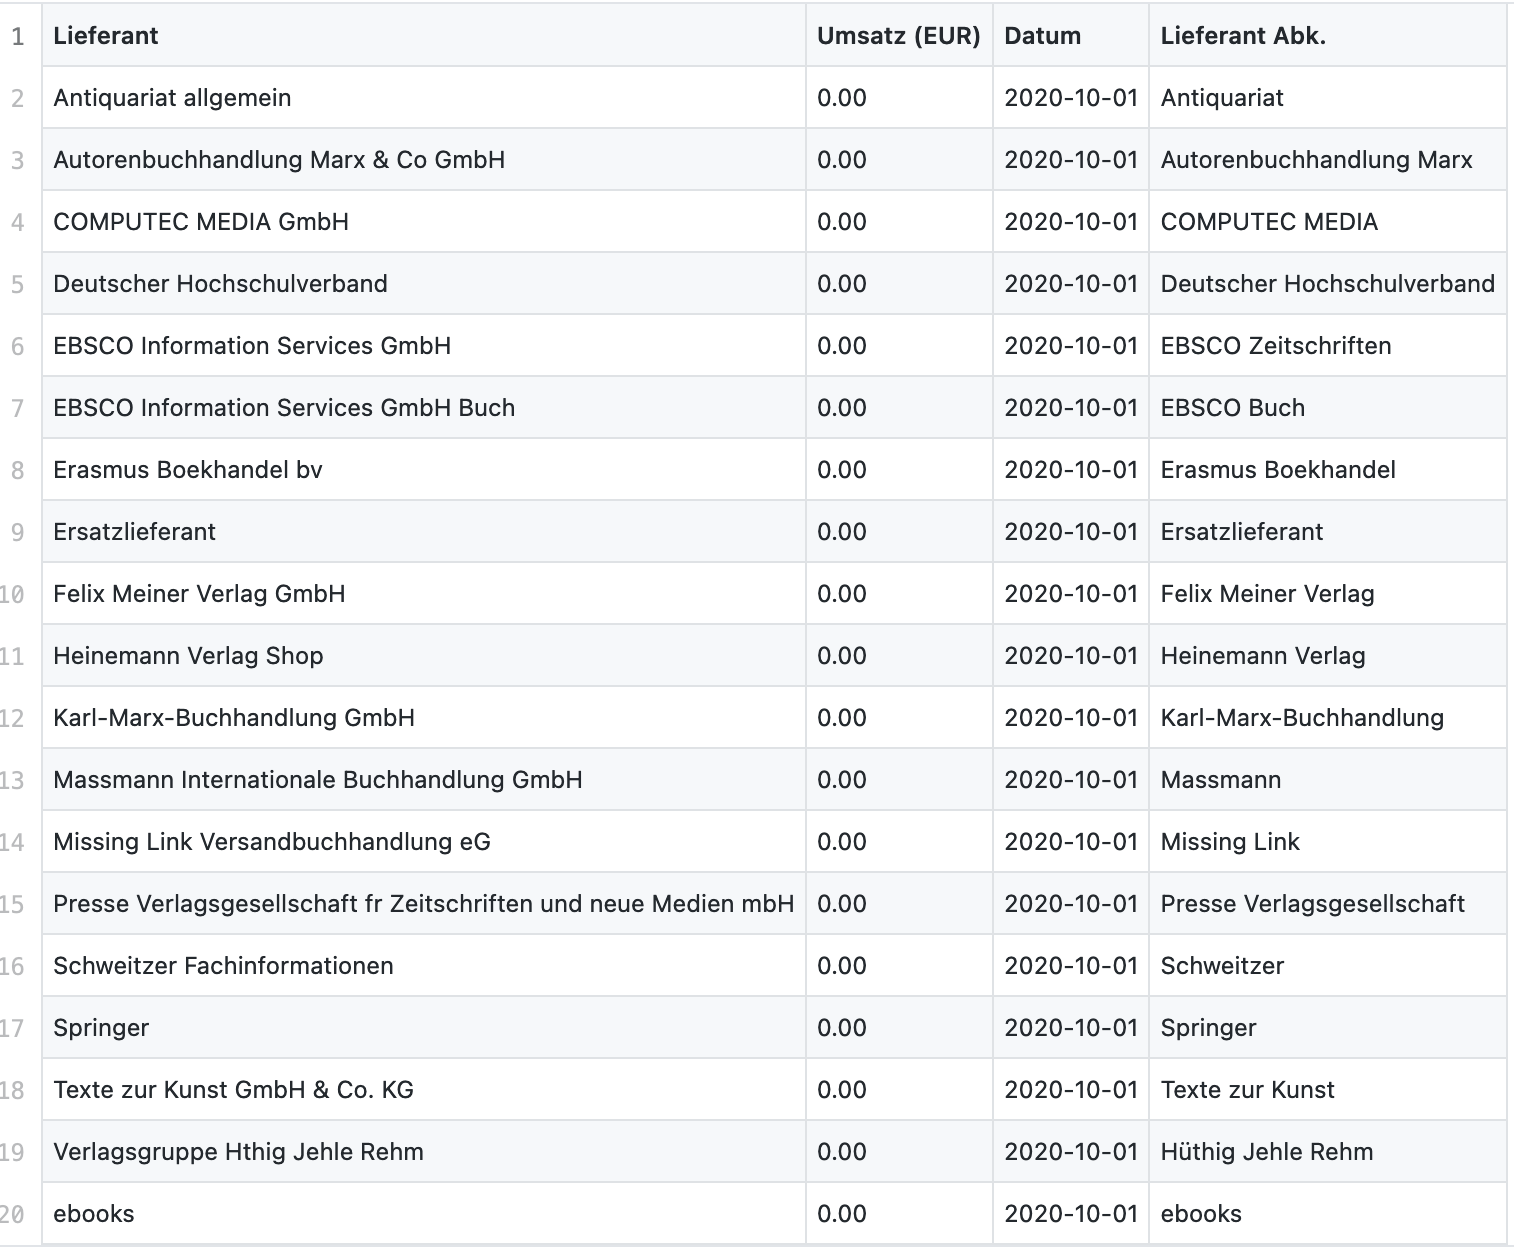
\includegraphics[width=6.5cm, height=7.0cm]{umsatz_csv_bsp}
            \caption{Monatliche Umsatzübersicht nach Ablauf Teilsystem Import}
            \label{fig:umsatzuebersicht_csv}
    \end{figure}
    
    \noindent
    \textit{Teilsystem 2 Datenbearbeitung}

    Das Teilsystem 2 hat als Ziel die Daten für die Darstellung im Dashboard vorzubereiten. Der weitere Zweck dieses
    Teilsystem ist es, die Vorbereitung der Daten von der Erstellung der Datenvisualisierungen zu trennen. Ein Grund hierfür
    ist, den Programmcode im Teilsystem 3 nicht mit dem Programmcode der Datenmanipulation zu überfrachten. Ebenfalls haben Überlegungen
    der Latenzzeit eine Rolle gespielt. Deswegen werden in dem Teilsystem Datenbearbeitung Daten mit pandas so bearbeitet, 
    dass entweder Teilmengen der eigentlichen Daten oder Ergebnisse mathematischer Operationen durch das Teilsystem 3 
    zu Datenvisualisierungen nur noch weiterverarbeitet werden müssen. Die Vorbereitung der Daten umfasst einzelne Berechnungen 
    wie \texttt{mean()} oder \texttt{sum()}. Ferner werden im Teilsystem 2 die Sortierung, Gruppierung, Filterung der 
    Daten nach bestimmten Aspekten vollzogen, die in den Anwendungsfällen formuliert sind.
    
    Für das Teilsystem Datenbearbeitung ist das Modul \texttt{data\_prep} zentral. Die Klassenstruktur dieses Moduls ist eine 
    Basisklasse von der vier Kindklassen erben. Es gibt Kindklassen für Umsatz und Budget-Daten, für Bestands- und Neuerwerbungsdaten, für Daten der Ausleihe und 
    der Lesesaalnutzung. Aufgrund der ähnlichen Datenstruktur der Umsatz- und Budgetdaten genügt eine Klasse für beide.
    Der Gesamtbestand und die monatlichen Neuerwerbungen berufen sich auf denselben Datenbestand, so dass hier ebenfalls auf eine Aufteilung auf mehrere Klassen verzichtet wurde.
    Für jede Kindklasse wurden Methoden geschrieben, die auf den spezifischen Bibliotheksdaten verschiedene Manipulationen ausführen.
    Die Ergebnisse werden von jeder Methode zurückgeben. \autoref{fig:classes data_prep} zeigt die Basisklasse und die vier Kindklassen mit ihren Methoden.


    \begin{figure}[H]
        \centering
            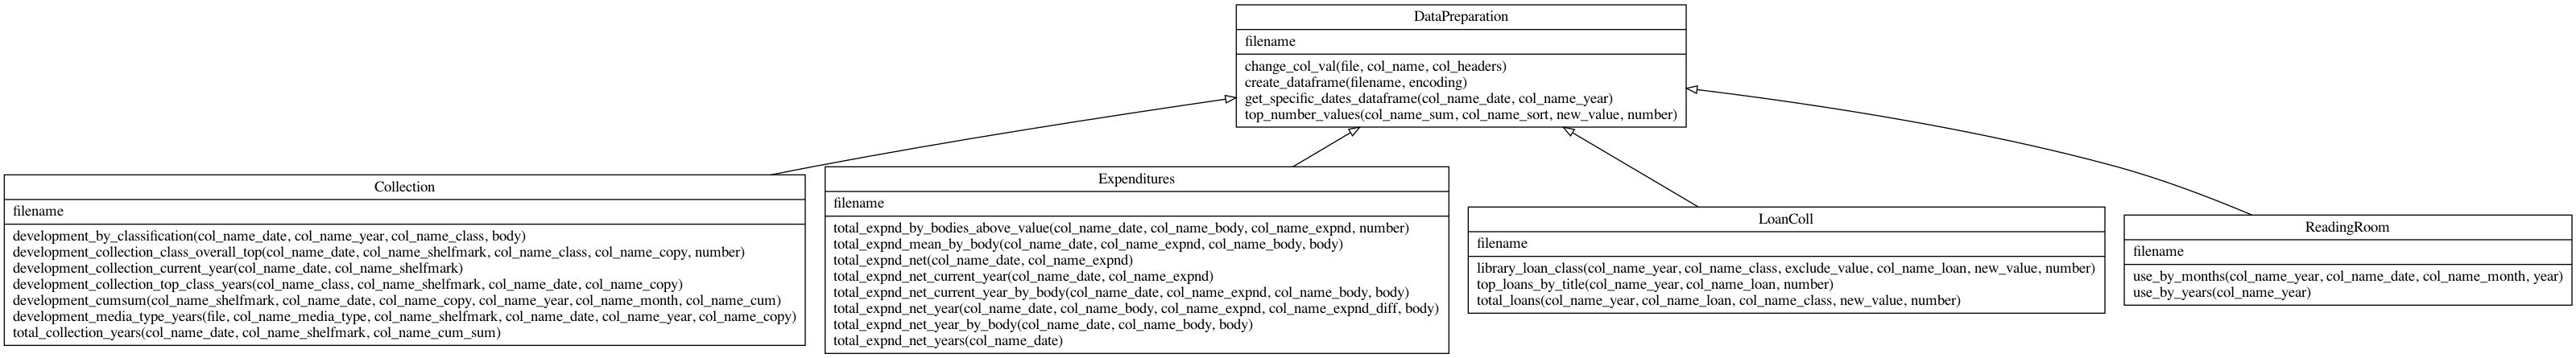
\includegraphics[width=15cm, height=4.5cm]{data_prep}
            \caption{Klassendiagramm - Teilsystem Datenbearbeitung}
            \label{fig:classes data_prep}
    \end{figure}

    Der Ablauf innerhalb des Teilsystems besteht aus zwei Schritten.\\
    (1) Das Laden der einzelnen csv-Dateien aus dem Zielverzeichnis wird durch die Methode \texttt{create\_dataframe} der Basisklasse geregelt.
    Es wird noch einmal sichergestellt, dass die Daten in einem Zeichenformat wie utf-8 in das pandas Dataframe geladen werden.
    Beim Aufrufen des Konstruktor beziehungsweise der \texttt{init}-Methode der Klasse wird die Methode \texttt{create\_dataframe} 
    automatisch mit aufgerufen. Da die Methode und die Konstruktor-Properties der Basisklasse mit vererbt werden, kann in den Kindklassen das Objekt ebenfalls mit dem 
    pandas Dataframe initiiert werden. Die Objekte werden im nächsten Schritt durch die spezifischen Methoden der Kindklassen bearbeitet.\\
    (2) Das Ergebnis der Manipulation der pandas Dataframes ist auf die Darstellung der Daten im Dashboard ausgerichtet. Als Input der einzelnen Methoden der
    Kindklassen werden verschiedene Parameter verlangt, mit denen dann der Dataframe entweder manipuliert oder auf ihm Berechnungen ausgeführt werden können. 
    Um die Datenpreparation zu erreichen, können verschiedene Transformationsschritte auf den Daten ausgeführt werden. 
    Die Rückgabewerte der Methoden sind veränderte pandas Dataframes, pandas Series oder ein Ergebnis einer mathematischen Operation.
    
    % Bei der folgenden Methode interessieren für die Darstellung im Dashboard nur die Umsatz/Budget-Daten für spezifische Datums-Daten. Hintergrund ist der, dass die 
    % monatlichen Umsatz- und Budgetdaten im Jahr akkumuliert werden. Wenn das Budget und der Umsatz nur Jahresweise dargestellt werden sollen, 
    % interessieren dementsprechend nur die Datensätze jeweils vom Dezember beziehungsweise vom aktuellen Monat im Jahr.
    

    % \begin{lstlisting}[language=Python, caption=Python example]
        
    %     def total_expnd_net_years(self, col_name_date):
    %         ...
    %         self._df = self.get_specific_dates_dataframe(col_name_date)
    %         return self._df

    % \end{lstlisting}
    

    % Die Methode \texttt{total\_expnd\_net\_years} der \texttt{Expenditures}-Klasse gibt nach einem Transformationsschritt einen pandas Dataframe zurück.
    % Der Transformationsschritt beinhaltet die Filterung des Dataframes nach spezifischen Werten in der Spalte des übergebenden Spaltennamens.
    % Zu diesem Zweck wird noch die Methode\\
    % \texttt{get\_specific\_dates\_dataframe} aufgerufen. 
    Anhand der folgenden Methode soll der letzte Schritt verdeutlicht werden.
    Die Methode \texttt{total\_expnd\_net\_current\_year} der \texttt{Expenditures}-Klasse bestimmt im Allgemeinen die Summe von Werten einer Spalte, gefiltert
    nach einem Wert einer anderen Spalte eines pandas Dataframes. Mit dieser Methode soll so zum Beispiel konkret der Gesamtumsatz des laufenden Jahres berechnet
    werden.

    \begin{lstlisting}[language=Python, caption=Beispiel Methode Exenditures class]
    def total_expnd_net_current_year(self, col_name_date, col_name_expnd):
        ... 
        self._date_max = self._df[col_name_date].max()
        self._df = self._df.set_index(col_name_date)
        self._df = self._df.loc[self._date_max]

        return self._df[col_name_expnd].sum()  
    \end{lstlisting}

    Als Input erwartet die Methode in der Methodensignatur zwei Spaltennamen als Parameter: den Namen der Datumspalte \texttt{col\_name\_date} nach der gefiltert wird
    und den Namen der Umsatz-Spalte auf der die Berechnung stattfindet.
    \texttt{col\_name\_expnd}. Der Transformationsprozess im Methodenkörper teilt sich in drei Schritte auf. Da die monatlichen Umsatzdaten im Jahr als 
    akkumulierte Daten vorliegen, interessieren nur die letzten vorhandenen Datensätze des laufenden Jahres. Deswegen
    wird nach diesen gefiltert und ein Dataframe von diesen erstellt. Dementsprechend wird mit der pandas-Funktion \texttt{max()} 
    der maximale Wert in der Datumsspalte zunächst bestimmt und der Variable \texttt{\_date\_max} zugewiesen. Danach wird die Datumsspalte als Index gesetzt. 
    Im dritten Schritt wird der Dataframe mit den Reihen, die der Variable \texttt{\_date\_max} entsprechen, erstellt. Dies geschieht mit der pandas-Funktion \texttt{.loc}, die
    auf den Index der Reihen des Dataframes zugreift. Zum Schluss wird auf Basis der Umsatz-Spalte des Dataframes die Summe mit der pandas-Funktion \texttt{sum()} berechnet 
    und als Rückgabewert zurückgeliefert. Der Rückgabewert kann nun vom Telsystem 3 Darstellung weiterverarbeitet werden.\\


    \noindent
    \textit{Teilsystem 3 Darstellung}\\
    Für die Erschaffung des Dashboards mit seinen Datenvisualisierungen und Interaktionen ist das Teilsystem Darstellung verantwortlich.
    In ihm werden die Ergebnisse des Teilsystems 2 zu Datenvisualisierungen verarbeitet und die Logik für die Darstellung dieser Datenvisualisierung 
    in einem Dashboard bereitgestellt.
    %In ihm werden die Datenvisualisierungen mit den den Ergebnissen aus dem Teilsystem Datenbearbeitung
    %geschaffen. 
    Dazu werden die Bibliothek Plotly Express für die Datenvisualisierungen und die Bibliothek Dash zur Umsetzung des Dashboards genutzt. 
    
    Aufgrund der Vielzahl an Datenvisualisierungen wurde sich gegen eine Single-Page-Lösung entschieden. Deswegen besteht das Dashboard
    aus drei einzelnen Tabs. Die Struktur der Dashboard-App entspricht einem Multi-App-Dashboard. 
    % Aufgrund der vielen Code-Blöcke tendieren Dashboards-Apps, die mit Dash geschrieben wurden zur Unübersichtlichkeit.
    
    Es gibt verschiedene Möglichkeiten Multi-App-Dashboard-Projekte zu strukturieren. Für das vorliegende Projekt wurde sich für die in \autoref{fig:dash structure}
    gezeigte Struktur entschieden.

    \begin{figure}[H]
        \centering
            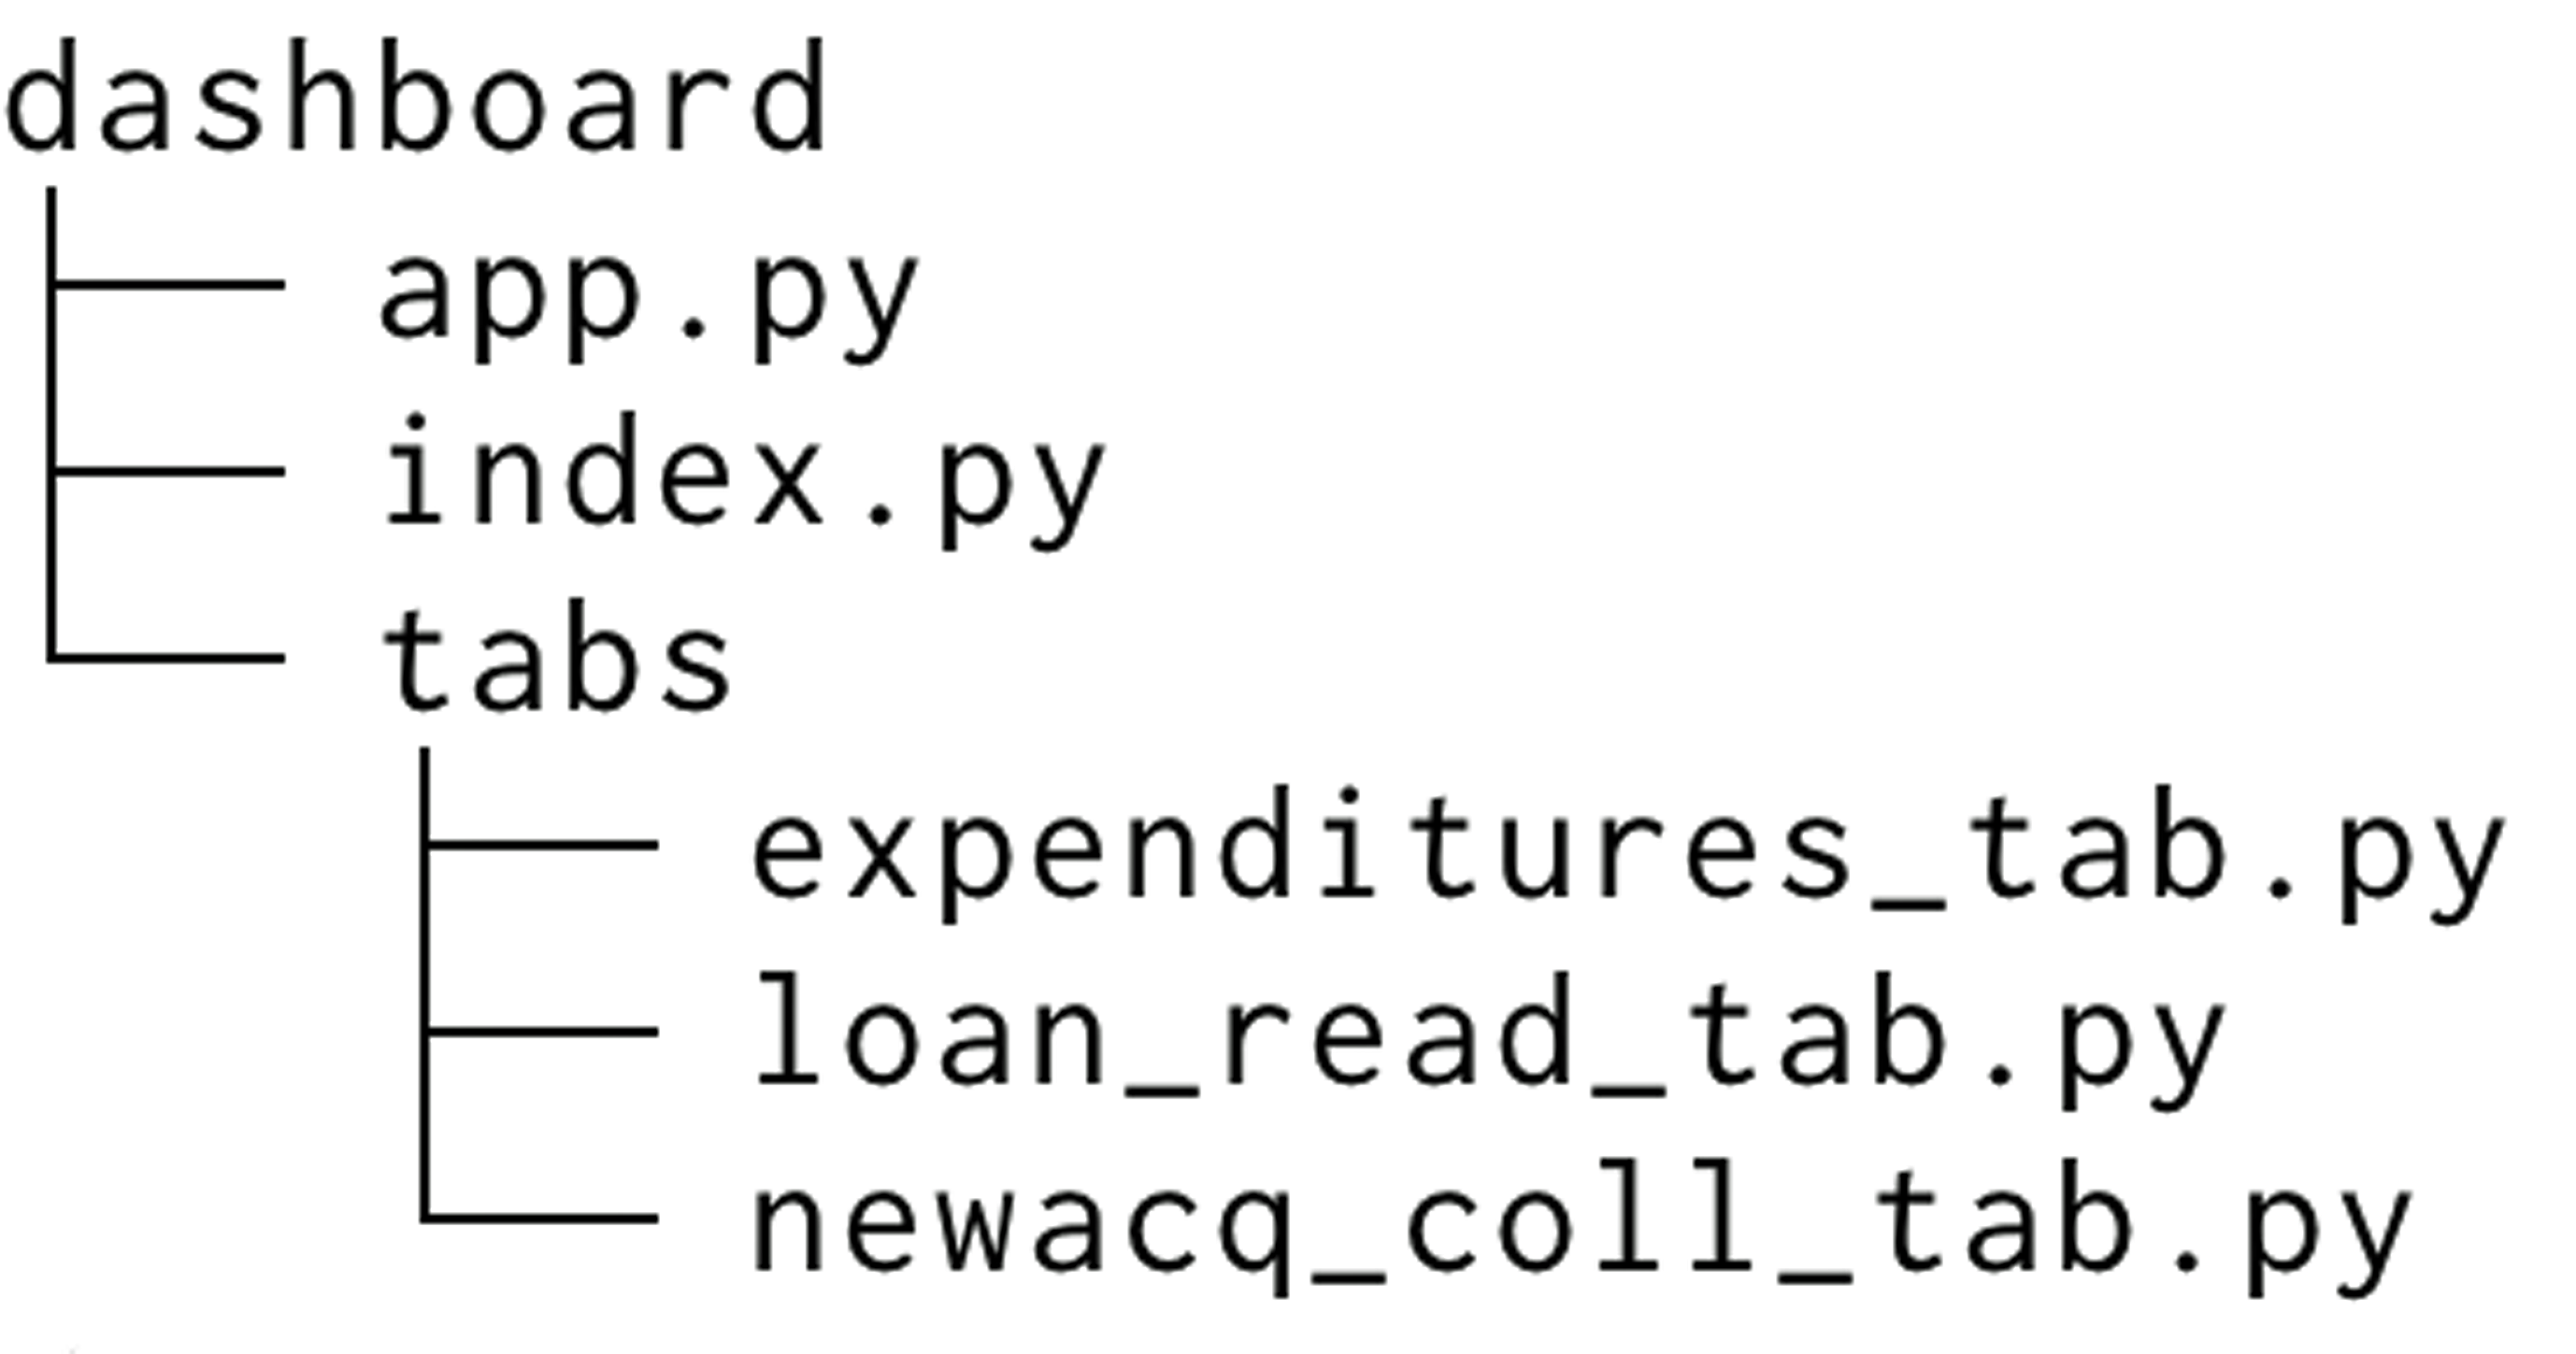
\includegraphics[width=6cm, height=3.5cm]{dash_struc}
            \caption{Struktur Dash Multi-Page App}
            \label{fig:dash structure}
    \end{figure}
    
    Dies entspricht einer der Möglichkeiten, wie sie auf der Webseite von Dash für Multi-App-Projekte vorgeschlagen werden \cite[vgl.][]{plotly_url_2021}.
    
    Die einzelnen Tabs wurden versucht inhaltlich um bibliothekarische Tätigkeiten zu gruppieren. So werden in der \texttt{expenditures\_app.py}
    Datenvisualisierungen erstellt, die Budget- und den Umsatzdaten visualisieren, während mit Hilfe der \texttt{loan\_read\_app.py}
    Ausleih- und Lesesaalnutzungsdaten dargestellt werden. Mit der \texttt{newacq\_coll\_app.py} wird ermöglicht Daten aus dem Bereich der Bestandsentwicklung und der 
    Ausleihe Daten zu präsentieren.

    Für jeden Tab gibt es eine separate Datei. Jede einzelne Tab-Datei besteht einerseits aus mehreren Funktionen, die mit der Bibliothek Plotly Express \texttt{Plotly Graph Objects} erzeugen.
    Andererseits bestehen die Dateien aus mehreren verschiedenen Funktionen für die Dash-Komponenten wie zum Beispiel Dropdown-Menüs, Cards oder Diagrammen. 
    Die Funktionen der Dash-Komponenten binden die Funktionen der \texttt{Plotly Graph Objects} so ein, dass die \texttt{Plotly Graph Objects} im Dashboard zur Anzeige gebracht werden können. 
    Weiterhin sind die Dash-Komponenten zum Teil mit Decorator-Callback-Funktionen verknüpft, die es ermöglichen mit dem Dashboard zu interagieren. 
    So bieten zwei Tabs des Dashboards die Möglichkeit an über ein Dropdown-Menü eine Auswahl der Daten zu treffen,
    die angezeigt werden sollen.

    Neben den Funktionen für die Dash-Komponenten und der \texttt{Plotly Graph Objects}, werden in den tab-Dateien noch die Objekte aus dem Modul \texttt{data\_prep} 
    instantiiert und die Methoden der Kindklassen aus diesem Modul auf diese angewendet. In der Regel ... Entweder innerhalb der Plotly-Funktionen oder außerhalb. Um die
    Daten interaktiv zu machen, mussten einige Objekte innerhalb der Funktionen initialisiert und bearbeitet werden. Dabei drehte es sich um Filterungen nach bestimmten Aspekten.


    Schematisch zeigt die \autoref{fig:process tab} den Ablauf in den Tab-Dateien mit callback-Funktionen \texttt{index.py}.
    
    \begin{figure}[H]
        \centering
            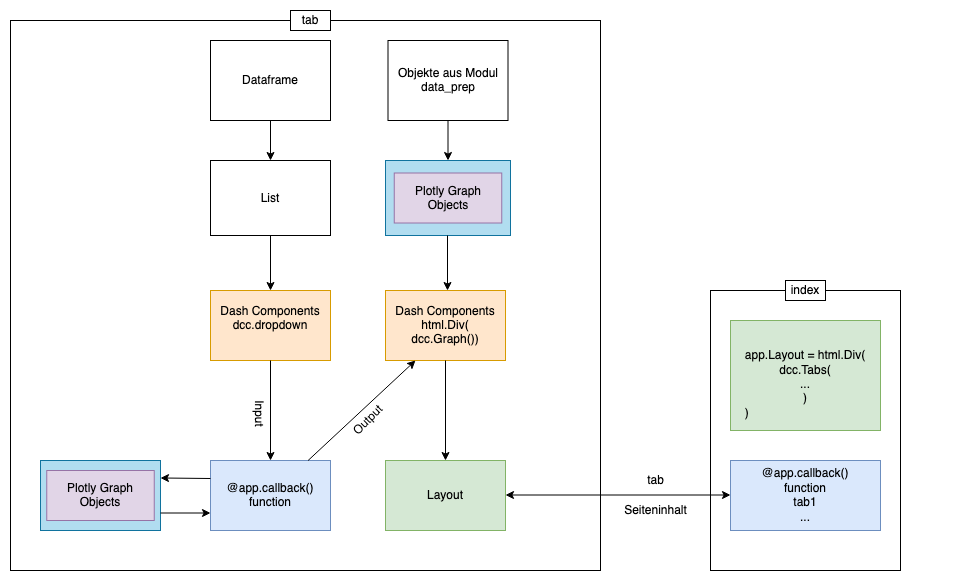
\includegraphics[width=15cm, height=12cm]{ablauf_dash}
            \caption{Ablauf Tab}
            \label{fig:process tab}
    \end{figure}

    In den Funktionen, die \texttt{Plotly Graph Objects} erzeugen, werden diese bearbeiteten Objekte als Parameter von Plotly Express Methoden entgegengenommen 
    und mit diesen Parametern \texttt{Plotly Graph Objects} erzeugt. Parameter, die zum Beispiel die x- und y-Achse bei Balken -und Liniendiagrammen
    festlegen, müssen dabei mit übergeben werden. Weitere Parameter, die das Layout festlegen, sind dagegen optional.
    
    Im folgenden Beispiel wird in der Funktion \texttt{fig\_total\_expnd} ein horizontal gekipptes Balkendiagramm mit dem Dataframe \texttt{df\_total\_expnd}, 
    der x-Achse 'Umsatz (EUR)' und y-Achse 'Datum' durch den Aufruf der Funktion \texttt{bar} erzeugt und der Variable \texttt{fig} zugewiesen. 

    \begin{lstlisting}[language=Python, caption=Funktion fig\_total\_expnd() Auszug 1]
    def fig_total_expnd():
        ...
        fig = px.bar(df_total_expnd,
            x='Umsatz (EUR)',
            y='Datum',
            orientation='h',
            ...
        )
        ...
    \end{lstlisting}
    
    Ebenfalls können \texttt{Plotly Graph Objects} noch durch andere Funktionen von Plotly Express bearbeitet werden. 
    So kann durch die \texttt{update\_layout}-Funktion der Achsentitel, Höhe und Breite der Datenvisualisierung festgelegt werden.

    \begin{lstlisting}[language=Python, caption=fig\_total\_expnd() Auszug 2]  
    def fig_total_expnd():
        ...
        fig.update_layout(title_x=0.5,
            xaxis_title='Umsatz in Euro',
            yaxis_title='Jahr',
            height=500)
        fig.update_xaxes(nticks=20)         
        return fig
    \end{lstlisting}

    Beispielhaft werden hier der Titel der x- und y-Achse, sowie die
    Größe des Diagramm-Objektes festgelegt. Schließlich wird noch die x-Achse mit der Funktion \texttt{update\_xaxes} skaliert.
    Als Rückgabewert der Funktion wird das \texttt{Plotly Graph Object} zurückgegeben.

    Diese Funktionen werden dann bei der Erstellung von den \texttt{HTML-Div-Components} mit Dash aufgerufen. In den Funktionen,
    die diese \texttt{HTML-Div-Components} als Rückgabewert haben, wird von der \texttt{Graph-Component} der \texttt{dash\_core\_components}
    die Funktion zur Erstellung des \texttt{Plotly Graph Object} aufgerufen. Die \texttt{Graph-Component} rendert interaktive Datenvisualisierungen unter Verwendung der Open-Source-JavaScript-Grafikbibliothek plotly.js.
    Ebenfalls wird von der \texttt{Graph-Component} eine 
    \texttt{id} als Argument entgegengenommen. Diese ist unter anderem wichtig für die Callback-Funktionen. 
    

    \begin{lstlisting}[language=Python, caption={html\_fig\_total\_expnd()}] 
    def html_fig_total_expnd():
    ...
    return html.Div(
        [
            html.Div(
                [
                    dcc.Graph(
                        id='gesamtumsatz',
                        figure=fig_total_expnd()
                    ),
                ], className="six columns chart_div", style={'margin-top': '20px', 'margin-left': '10px'}
            ),
        ]
    )
    \end{lstlisting}

    Diese werden schließlich in der Layoutfunktion der Tab-Datei in einem Div-Objekt zusammengefasst.
    
    Die Callback-Funktionen wurden nur in zwei Tab-Dateien implementiert. 
    In der \texttt{expenditures\_app.py} sind zum Beispiel jeweils zwei Diagramme und Zahlenwerte von den Werten 
    einer Dropdown-Liste abhängig. 

    Der Einstiegspunkt zur Ausführung des Dashboards ist die Datei \texttt{index.py}. Mit dieser Datei wird das Dashboard mittels \texttt{Flask-Webserver}
    gestartet. Zur Vermeidung zirkulärer Importe ist die Dash-Instanz in der separaten \texttt{app.py} definiert\cite[vgl.][]{plotly_url_2021}.
    Die \texttt{index.py} definiert zudem das Layout des gesamten Dashboards. Hier wird auch die Anzahl der Tabs festgelegt. Die
    Decorator-Callback-Funktion \texttt{@app.callback()} steuert die Auswahl der Tabs und ruft die jeweiligen Tabs auf.



    %\textit{Standardbericht}\\

\section{Dashboard}

  

    \subsection{Umgesetzte Anforderungen}
    Folgende Must-Anforderungen wurden erfüllt.
    R1, R2, R3, R4, R5, R7
    F1, F4, F5, F12
    NF5, NF6, 
    \subsection{Funktionsweise}
    \textit{Dashboard}
    Das Layout des Dashboards besteht aus drei Tabs. Diese wurden nach den Bereichen der Bibliothek aufgeteilt. Diese Aufteilung erschien als sinnvoll,
    da auf grafische Oberfläche nicht überladen werden sollte.
    Nach dem der Webserver gestartet wurde, landet man im Tab1 und bekommt die dort verankerten Inhalte zu sehen.
    Tabs sind als Reiter oben auf der Webseite angesiedelt.
    Drauf klicken und man gelangt auf den Inhalt desa Tabs (Seite)
    
    Fast allen Diagrammen wohnt inne, dass man aus der Legende auswählen kann welche Elemente angezeigt bzw. nicht angezeigt werden sollen.
    mitunter auch hover elemente, wenn über die einzelnen Balken oder Linien mit der Maus gefahre 
    
    Tab1 - Umsatz und Budget
    
    Bild Tab1
    Was ist dargestellt:
    
    zwei Diagramme mit 
        Anzeige des Gesamtumsatz nach Jahren und nach Lieferanten ->  horizontalestapeltes Balkendiagramm
        umsatzstärkste Lieferanten (Top 7) Verteilung in Prozent (Kreisdiagramm)
        
    zwei Diagramme mit interaktiver Auswahl eines Lieferanten über Dropdownmenü
        Anzeige des Gesamtumsatzes nach Jahren für de ausgewählten Lieferanten (Liniendiagramm)
        Anzeige des Umsatzes pro Monat für das laufende Jahr (Balkendiagramm)
    
    zwei Diagramme mit
        Anzeige des Gesamtbudgets nach Jahren und nach Kostenstellen 
        Anzeige kostenintesive (Top 7) Kostenstellen
        
    
    vier Karten mit
        Zahl des Gesamtumsatzes
        Zahl des Umsatzes im Jahr
        Zahl des Umsatzes im laufenden Jahrs für den einzelnen Lieferanten (gekoppelt mit Dropdown-Auswahl)
        Durchschnittlicher Umsatz des Lieferanten (gekoppelt mit Dropdown-Auswahl)
    
    
    
    
    
    Tab2 - Lesesaal und Ausleihe
    
    Bild Tab2
    
    zwei Diagramme mit
        Anzeige der Nutzer:innen nach Jahren und nach Service-Zeiten (gruppiertes Balkendiagramm)
        Anzeige der Nutzer:innen nach Monaten und nach Service-Zeiten für das laufende Jahr.
        
     ein Diagramm mit
        Anzeige der Ausleihanzahl nach Jahren (horizontales Balkendiagramm)
    
    Tab3 - Bestand
    
    Bild Tab3

    
     



\section{Bewertung}
zur Datenlage 
Ausleihdaten nur auf Zuruf, mtl. Daten bekommen wir erst seit 2021 zu geschickt.
kumulative Daten bei Umsatz/Budget
fehlen der UmsatzDaten für Datenbanken müsste nochmal händisch nachgetragen werden (ca. 20.000 Euro)
Fehlen der Buchservice-Daten (Subito, ...) -> keine Zeit
nur Daten die aus dem CBS/LBS  stammen
fehlen Daten der Online-Zeitschriften

dennoch:
gelungen, die vorhandenen Daten soweit zu importieren, dass mit diesen über das Dataframes Manipulationen und Berechnungen
durchgeführt werden können. Ebenso ist es gelungen eine grafische Oberfläche für die Diagramme anzubieten. Diese Diagramme
sind mit Plotly interaktiv. Es konnte auch ein bisschen interaktivität selber programmiert werden.

Es konnte gezeigt werden, das das gelingt\dots

Den größten Teil der Zeit hat die Datenanalyse gekostet (-> ähnlich Data Science Circle). 
pandas sehr mächtig und aber auch nicht trivial ist. Ziemlich gutes Tool für die Datenanaylyse darstellt.


